\edef\mychapter{Functions and Relations}
\edef\mychapterdate{June 18, 2024}

\chapter{\mychapter}
\section{Binary Relations}
Before we dive into functions, I'd like to spend some time talking about binary relations, as we will come to learn, functions are just a very special kind of relation. 
\begin{define}
	Let $\square$ be a binary relation. Then $\square\subseteq X \times Y$.\footnotemark 
	Then we say $x \,\square\, y$ \footnotemark if and only if $(x,y)\in \square$.
\end{define}
\footnotetext{$x$ is related to $y$ by $\square$}
\addtocounter{footnote}{1}
\footnotetext{The $\times$ here is a cartesian product; it means the set of all ordered pairs (x,y) where $x\in X$ and $y\in Y$.}

This definition of a binary relation might seem a bit confusing at first, but after pondering this for a second, this is, in fact, a very natural way to view a binary relation. 
Though the term binary relation is quite new, you've probably been working with binary relations in math your entire life. 

A good example would be the relation $\le$. For our purposes, I will represent this relation with the symbol $\triangle$, where
$a \,\triangle\, b$ if and only if $a\le b$.
Let us examine how this works.

First, we need to establish for what sets we are relating. For this example, I will use the natural numbers less than or equal to 3, so defining
$$S:=\{n\in\nat : n \le 3\},$$
we have $\triangle \subseteq S^2$.\footnote{$S^2=S\times S$}
Let's fix, for now, $a=1$. 
Then we find since 
$$1 \,\triangle\,1, \quad 1 \,\triangle\,2, \quad 1 \,\triangle\,3,$$
hence we find \textit{1 is related to 1, 2, and 3}; 
$$\{(1,1),(1,2),(1,3)\}\subseteq \triangle.$$
Repeating this exercise, we also find
$$2 \,\triangle\,2, \quad 2 \,\triangle\,3, \quad 3 \,\triangle\,3$$
hence
$$\{(2,2),(2,3),(3,3)\} \triangle$$
where we can conclude by stating
$$\triangle=\{(1,1),(1,2),(1,3),(2,2),(2,3),(3,3).\}$$

Interestingly enough, however, what we have done here is the exact opposite of how modern mathematicians define the greater than and less than operators to create ordered sets in more generality. 
A discussion of this is too complex for our purposes now, but if anyone is interested, I've left some links in the footnotes, for if anyone wants to learn more.\footnote{\href{https://proofwiki.org/wiki/Definition:Ordering}{https://proofwiki.org/wiki/Definition:Ordering}}

\section{Functions}
\subsection{Definition}
As I mentioned before, a function is just a type of relation, so in this section, we will explore what a function actually is from a more fundamental perspective.

\begin{define}
	Define relation $\square\,\subseteq X\times Y$. If
	\begin{enumerate}
		\item for every $x\in X$, there exists $y\in Y$ such that $(x,y)\in \square$,
		\item $(x,y)\in \square$ and $(x,z)\in \square$ implies $y=z$,
	\end{enumerate}
	then we say $\square$ is the graph\footnotemark
	that defines the function $f:X\to Y$, where $(x,y)\in\square$ implies $f(x)=y$.
	\label{def:function}
\end{define}
\footnotetext{Notice here that I'm not referring to the \textit{plot} of a function as you've seen in your previous classes. Instead, I'm talking about the underlying structure that connects inputs to outputs, sort of like a web. 
From now on, I will refer to the thing we draw as a plot to save some confusion.}

This definition might be a bit tough to swallow, but before diving into this, we should quickly review some vocabulary for functions. I assume many of you have never defined a function using the notation I've introduced above, so let's break that down first.

The statement $f:X\to Y$ can be read simply as a \textit{function $f$ from $X$ \textbf{to} $Y$} where $X$ is the \textbf{domain} and $Y$ is the \textbf{codomain}. 
You may have also seen a function be referred to as a \textit{mapping}\footnote{or a functional, depending on context} since all a function does is \textit{map} things from one set to another.

Now, with that out of the way, let's look at our conditions.
Looking at the first condition requires that every element in $X$ must have a corresponding element in $Y$. 
This matches what we should know about functions: that the function should be defined on its entire domain.
The next condition says that if $f(a)=b$, and $f(a)=c$, then $b=c$, or in other words, every input can have only one output.
You may have formulated this idea with a vertical line test in your previous math classes.
But that definition requires the function to have a graphical representation.
Since we know that the domain and codomain need not be sets of numbers, there exist functions that have no meaningful graphical representations.
What this definition does is that it generalizes that fact to a more general class of functions, even when we can't plot them.

But notice, nowhere in this definition of a function did we specify anything about the codomain of a function. 
With this, we can conclude that even if an element is in a function's codomain, it need not be related to anything in the domain.
This is important since we can define some functions $f(x)=g(x)=x^2$ for $f:\real\to\real$ and $g:\real\to\real^+$\footnote{Positive reals}, where both of these functions are well-defined under our definition of a function.
It's easy to tell the graph of the functions are equivalent, and using our prior knowledge, we conclude that the functions are equivalent\footnote{
If you are still unsure, just observe that the same inputs relate to the same outputs.}.
But since if two functions are equal, we should expect the functions to be defined equivalently, what we get is that $f\not\equiv g$, since the domains of $f$ and $g$ are different.

\begin{define}
	We call $f(A)$ the \textbf{image of $f$ under $A\subseteq X$}  if and only if
	$$f(A):=\{f(a) : a\in A\}.$$
\end{define}

This definition might seem very similar to the definition of the range that you might already be familiar with.
We will denote the range as $f(X)$ or the image of $f$ under the entire domain.
Now, contrast this definition of range with our definition of a codomain.
While not every element in a function's codomain needs to be related to an element in the domain, every element in a function's range must be related to an element in its domain.
This idea is highlighted in the figure \eqref{fig:function}, where the arrows between elements show the structure of the function's graph.
Since the element $f$ is unrelated to any element in $X$, we say $f$ is not in the range.\footnote{We note that $f(X)\subseteq Y$ for any well-defined function.}

\begin{figure}[h]
\centering
\resizebox{0.7\linewidth}{!}{
	\begin{tikzpicture}
		\filldraw[white] (-7,-3) rectangle (7,3);
			
		\draw (-3,0) ellipse (1.5 and 3) node[yshift=3.5cm] {$X$};
		
		\draw (3,0) ellipse (1.5 and 3) node[yshift=3.5cm] {$Y$};
		\draw (3,0.8) ellipse (1 and 1.9);
		\draw[thick, ->] (5.3,1.8) node[xshift=.8cm] {$f(X)$} -- (4.1,1.5);
		
		\node (a) at (-3,2) {\Large$a$};
		\node (b) at (-3,0) {\Large$b$};
		\node (c) at (-3,-2) {\Large$c$};
		
		\node (d) at (3,2) {\Large$d$};
		\node (e) at (3,0) {\Large$e$};
		\node (f) at (3,-2) {\Large$f$};
		
		\draw[thick,->] (a.east) -- (e.west);
		\draw[thick,->] (b.east) -- (e.west);
		\draw[thick,->] (c.east) -- (d.west);
		
		\draw (0,-4) node {$f:X\to Y$};

	\end{tikzpicture}}
	\caption{}
	\label{fig:function}
\end{figure}

\begin{define}
	We call $f^{-1}(B)$ the \textbf{preimage of $f$ under $B\subseteq Y$}, where
	$$f^{-1}(B):=\{x\in X : f(x)\in B\}.$$
\end{define}

We will not be using this definition that much in precalculus, but it is still a good one to know and will help us with the theorem in a later section.
A way we can understand this definition is if that $f^{-1}(B)$ is the set that contains all elements of $X$ that gets mapped to $B$.\footnote{Note: this operation \textit{is not} equivalent to the inverse of a function, we will discuss inverses in the next sections.}
We will note that $f^{-1}(Y)=X$. I will leave this as an exercise for you to check your understanding of this definition.

\begin{figure}[h]
\centering
\resizebox{0.7\linewidth}{!}{
	\begin{tikzpicture}
		\filldraw[white] (-7,-3) rectangle (7,3);
			
		\draw (-3,0) ellipse (1.5 and 3) node[yshift=3.5cm] {$X$};
		
		\draw (3,0) ellipse (1.5 and 3) node[yshift=3.5cm] {$Y$};
		\draw (-3,0.8) ellipse (1 and 1.9);
		\draw[thick, ->] (-5.3,1.8) node[left] {$f(\{e\})$} -- (-4.1,1.5);
		
		\node (a) at (-3,2) {\Large$a$};
		\node (b) at (-3,0) {\Large$b$};
		\node (c) at (-3,-2) {\Large$c$};
		
		\node (d) at (3,2) {\Large$d$};
		\node (e) at (3,0) {\Large$e$};
		\node (f) at (3,-2) {\Large$f$};
		
		\draw[thick,->] (a.east) -- (e.west);
		\draw[thick,->] (b.east) -- (e.west);
		\draw[thick,->] (c.east) -- (d.west);
		
		\draw (0,-4) node {$f:X\to Y$};

	\end{tikzpicture}}
	\caption{}
	\label{fig:preimage}
\end{figure}


\begin{ex}
	In this example, I'd like to demonstrate how to find the maximum possible domain and image for the function
	$$f(x):=\sqrt{x},$$ 
	such that 
	$$X\subseteq\real \jand f(X)\subseteq \real,$$
	where $X$ is the domain of $f$.
	The maximum possible domain is just simply the domain for the graph of a function for which we exclude every possible input that causes a function to be ill-defined. 
	Since we know $\sqrt{x}$ doesn't have real outputs for $x<0$, we let $X=[0,\infty)$. 
	Then, to find the image, with how $\sqrt{x}$ is defined, we only take the positive value of the two theoretically possible outputs hence, we find
	$$f(X)=[0,\infty).$$
\end{ex}
\begin{ex}
	In this example, let's find the maximum possible domain for 
	$$f(x):=\frac{x-1}{x^2+x-2}$$
	where $X$ is the domain and
	$$X\subseteq\real.$$
	Since this is a rational function, the only potential issue here is that $f$ will run into a divide by 0. We can see this is the case when $x=-2$. But this is only one of the possible issues we might run into with $f$. Therefore, to find the rest, we want to find $x$ such that
	$$x^2+x-2=0$$
	hence
	$$x^2+x-2=(x+2)(x-1)=0$$
	where we find when $x=1,-2$, the denominator is zero.
	Thus we define 
	$$X=\{x\in\real:x\neq1,-2\}.\footnotemark$$
	\footnotetext{
	Notice since $f(x)=\frac{x-1}{(x+2)(x-1)}$, so we might be inclined to say $f(x)=\frac{1}{x+2}$ and conclude $X=\{x\in\real:x\neq-2\}$. But this is indeed incorrect since when we divided out the $x-1$, we inadvertently divided by zero since we never excluded $x=1$ from our domain.}
	The image is slightly more difficult to find, so we will leave that for a future discussion.
\end{ex}


\subsection{Odd or Even}
\begin{define}
	Let $f: D \to \real$\footnotemark. We say $f$ is odd if and only if $f(-x)=-f(x)$.
	Furthermore, we say $f$ is even if and only if $f(-x)=f(x)$.	
\end{define}
\footnotetext{From now on, we will use $D$ to signify a domain in $\real$.}

Now, this may seem like a rather arbitrary definition, but rather than worry about the particular wording of this concept, just interpret this as any other mathematical notation or definition as if the wording bears no resemblance to its counterpart when used to refer to numbers. 

\begin{theorem}
\label{thm:ee}
	Let $f: D\to\real$ and $g: D\to\real$ be even functions. Then the following are true:
	\begin{enumerate}
		\item $f+g$ is even,
		\item $f\cdot g$ is even,
		\item $f-g$ is even,
		\item $\frac{f}{g}$ is even, for $g(x)\neq 0$ for all $x\in D$. 
	\end{enumerate}
\end{theorem}
\begin{proof}
	Since
	$$(f+g)(-x)=f(-x)+g(-x)=f(x)+g(x)=(f+g)(x)$$
	hence, the function $f+g$ is even, therefore proving (1).
	
	Then, using the same technique,
	$$(f\cdot g)(-x)=f(-x)\cdot g(-x)=f(x)\cdot g(x)=(f\cdot g)(x)$$
	hence proving (2).
	
	Let $h(x)=-1$. Then observe $h(-x)=h(x)=-1$, hence $h$ is even. Then
	$$(f-g)(x)=f(x)+h(x)g(x)$$
	Since $h\cdot g$ is even, we conclude that $f-g$ is also even, hence proving (3).
	
	Then since
	$$\paren{\frac{f}{g}}(x)=\frac{f(-x)}{g(-x)}=\frac{f(x)}{g(x)},$$
	we can conclude $\frac{f}{g}$ is even.
\end{proof}

\begin{theorem}
\label{thm:eo}
Let $f: D\to\real$ and $g: D\to\real$ be even and odd functions, respectively. Then
\begin{enumerate}
	\item $f\cdot g$ is odd
	\item $\frac{f}{g}$ is odd, for $g(x)\neq 0$ for all $x\in D$. 
\end{enumerate}
\end{theorem}
\begin{proof}
	The proof works similarly to how we proved theorem \eqref{thm:ee}.
	Since
	$$(f\cdot g)(-x)=f(-x)g(-x)=f(x)\cdot (-g(x))=-(f\cdot g)(x)$$
	hence proving $f\cdot g$ is odd.
	Then since
	$$\paren{\frac{f}{g}}(-x)=\frac{f(-x)}{g(-x)}=\frac{f(x)}{-g(x)}=-\paren{\frac{f}{g}}(x)$$
	Thereby proving the theorem.
\end{proof}
 We can actually reverse the functions in theorem \eqref{thm:eo} and get the same conclusion (the proof follows exactly as above).
 Notice, in theorem, \eqref{thm:eo}, we didn't mention anything about when these functions were added.
 This is because the odd or evenness of a function cannot be determined if nothing else is known about the function. Nevertheless, something interesting will happen, as we will explore soon.

\begin{theorem}
	\label{thm:oo}
	Let $f: D\to\real$ and $g: D\to\real$ be odd functions. Then the following are true:
	\begin{enumerate}
		\item $f+g$ is odd,
		\item $f\cdot g$ is even,
		\item $f-g$ is odd,
		\item $\frac{f}{g}$ is even, for $g(x)\neq 0$ for all $x\in D$. 
	\end{enumerate}
\end{theorem}
\begin{proof}
	Exercise.
\end{proof}

\begin{theorem}
	Let $f: D\to\real$ be any arbitrary function. Then there exists $g:D\to\real$ and $h:D\to\real$, even and odd respectively such that
	$$f=g+h$$
\end{theorem}
\begin{proof}
	Define
	$$g(x)=\frac{f(x)+f(-x)}{2}$$
	$$h(x)=\frac{f(x)-f(-x)}{2}$$
	Then the sum $g+h$ is trivially $f$. 
	To prove $g$ is even:
	$$g(-x)=\frac{f(-x)+f(-(-x))}{2}=\frac{f(-x)+f(x))}{2}=g(x).$$
	And $h$ is odd:
	$$h(-x)=\frac{f(-x)-f(-(-x))}{2}=\frac{f(-x)-f(x))}{2}=-\frac{f(x)-f(-x)}{2}=-h(x).$$
	Since our definitions of $g$ and $h$ are even and odd, respectively, this concludes our proof of the theorem. 
\end{proof}

We will conclude our discussion of odd and even functions in this lesson and pick up on their applications in future lessons. For now, just remember the definition of this idea and its basic properties. 

\subsection{Compositions and Inverses}
\begin{define}
	Let $f: X\to Y$ be a function. $f$ is said to be \textbf{one-to-one (injective)} if for every $x_1,x_2\in X$ such that $f(x_1)=f(x_2)$ implies $x_1=x_2$ or equivalently, $x_1\neq x_2$ implies $f(x_1)\neq f(x_2)$.
\end{define}
\begin{define}
	Let $f: X\to Y$ be a function. $f$ is said to be \textbf{onto $Y$ (surjective)} if for every $y\in Y$, there exists $x\in X$ such that $f(x)=y$.
\end{define}
\begin{define}
Let $f:X\to Y$ be one-to-one and onto $Y$. Then $f$ is said to be a \textbf{bijection}.	
\end{define}

The mathematical jargon may be a bit tough to comprehend, but let's break each down individually. 

A one-to-one function, simply put, is a function where there can be a maximum of \textbf{one} input that maps to each output. 
\begin{figure}[h]
\centering
\resizebox{0.7\linewidth}{!}{
	\begin{tikzpicture}
		\filldraw[white] (-7,-3) rectangle (7,3);
			
		\draw (-3,0) ellipse (1.5 and 3) node[yshift=3.5cm] {$X$};
		
		\draw (3,0) ellipse (1.5 and 3) node[yshift=3.5cm] {$Y$};
		\draw[thick, ->] (5.3,1.8) node[xshift=.8cm] {$f(X)$} -- (4.1,1.5);
		
		\node (a) at (-3,2) {\Large$a$};
		\node (b) at (-3,0) {\Large$b$};
		
		\node (d) at (3,2) {\Large$d$};
		\node (e) at (3,0) {\Large$e$};
		\node (f) at (3,-2) {\Large$f$};
		
		\draw[thick,->] (a.east) -- (e.west);
		\draw[thick,->] (b.east) -- (d.west);
	\end{tikzpicture}}
	\caption{one-to-one function}
	\label{fig:inject}
\end{figure}
As in figure \eqref{fig:inject}, each output has a maximum of one connection.
A common way to visualize a real one-to-one function on a plot is that a one-to-one function passes a horizontal line test. 
Like the vertical line test, if for every horizontal line, the line only passes through the plot at most once, then the function is one-to-one. If the function wasn't defined on a number line, the horizontal line test wouldn't apply, but it's still a useful test for when we are getting still getting used to these ideas.

An onto function is a function where the image is equal to the codomain. As you can see in the figure \eqref{fig:sur}, every element in $Y$ has at least one corresponding element in $X$ that maps to it. 

Then, when you put these together, the resulting function passes the horizontal line test and maps to every element in $Y$, as in figure \eqref{fig:bi}, we get a bijection.
\begin{figure}[h]
\centering
\resizebox{0.7\linewidth}{!}{
	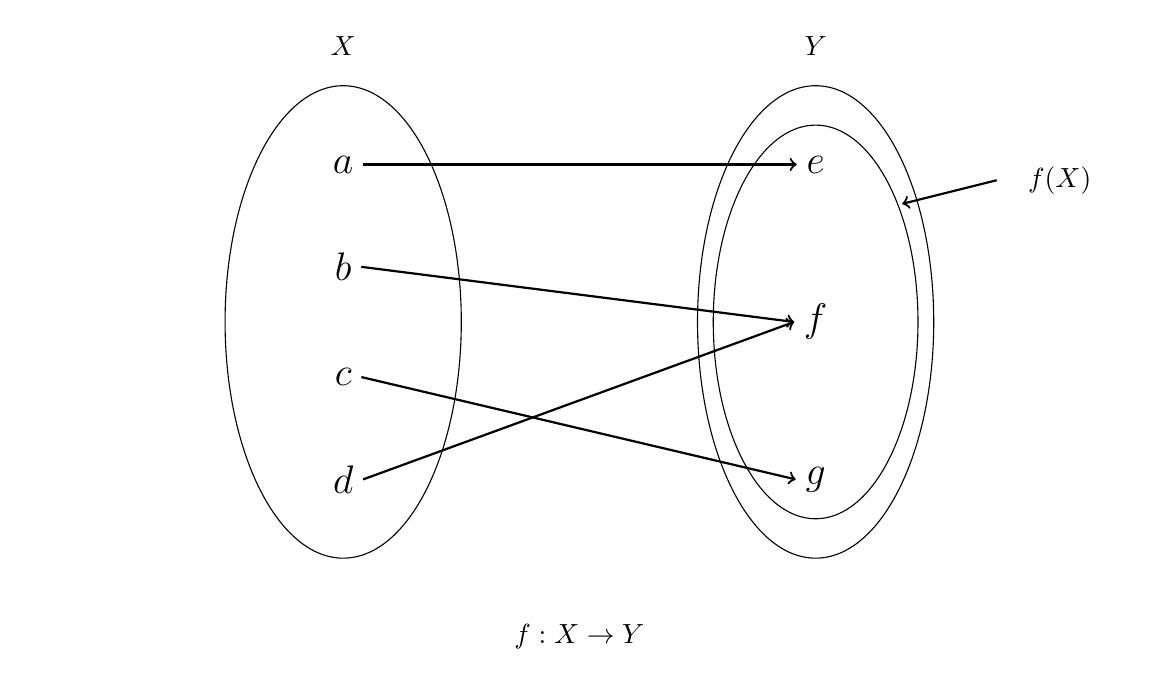
\begin{tikzpicture}
		\filldraw[white] (-7,-3) rectangle (7,3);
			
		\draw (-3,0) ellipse (1.5 and 3) node[yshift=3.5cm] {$X$};
		
		\draw (3,0) ellipse (1.5 and 3) node[yshift=3.5cm] {$Y$};
		\draw (3,0) ellipse (1.3 and 2.5);
		\draw[thick, ->] (5.3,1.8) node[xshift=.8cm] {$f(X)$} -- (4.1,1.5);
		
		\node (a) at (-3,2) {\Large$a$};
		\node (b) at (-3,.7) {\Large$b$};
		\node (c) at (-3,-.7) {\Large$c$};
		\node (d) at (-3,-2) {\Large$d$};
		
		\node (e) at (3,2) {\Large$e$};
		\node (f) at (3,0) {\Large$f$};
		\node (g) at (3,-2) {\Large$g$};
		
		\draw[thick,->] (a.east) -- (e.west);
		\draw[thick,->] (b.east) -- (f.west);
		\draw[thick,->] (c.east) -- (g.west);
		\draw[thick,->] (d.east) -- (f.west);
		
		\draw (0,-4) node {$f:X\to Y$};

	\end{tikzpicture}}
	\caption{}
	\label{fig:sur}
\end{figure}

\begin{figure}[h]
\centering
\resizebox{0.7\linewidth}{!}{
	\begin{tikzpicture}
		\filldraw[white] (-7,-3) rectangle (7,3);
			
		\draw (-3,0) ellipse (1.5 and 3) node[yshift=3.5cm] {$X$};
		
		\draw (3,0) ellipse (1.5 and 3) node[yshift=3.5cm] {$Y$};
		\draw (3,0) ellipse (1.3 and 2.5);
		\draw[thick, ->] (5.3,1.8) node[xshift=.8cm] {$f(X)$} -- (4.1,1.5);
		
		\node (a) at (-3,2) {\Large$a$};
		\node (b) at (-3,0) {\Large$b$};
		\node (c) at (-3,-2) {\Large$c$};
		
		\node (d) at (3,2) {\Large$d$};
		\node (e) at (3,0) {\Large$e$};
		\node (f) at (3,-2) {\Large$f$};
		
		\draw[thick,->] (a.east) -- (e.west);
		\draw[thick,->] (b.east) -- (f.west);
		\draw[thick,->] (c.east) -- (d.west);
		
		\draw (0,-4) node {$f:X\to Y$};

	\end{tikzpicture}}
	\caption{}
	\label{fig:bi}
\end{figure}

With this newfound vocabulary, we are one step closer to talking about inverses, but before we do, we must talk about functional composition.
When we compose functions, what we do is take the output from one function and put it into another function.
Because of some of the properties of this operation, the symbol we use for this looks very similar to multiplication.\footnote{If you ever take linear algebra, functional composition distributes on addition very similarly to how multiplication does. It also has an interesting connection to matrix multiplication, which is where I assume we get the symbol from (I'm not completely sure).}

\begin{figure}[h]
\centering
\resizebox{0.8\linewidth}{!}{
	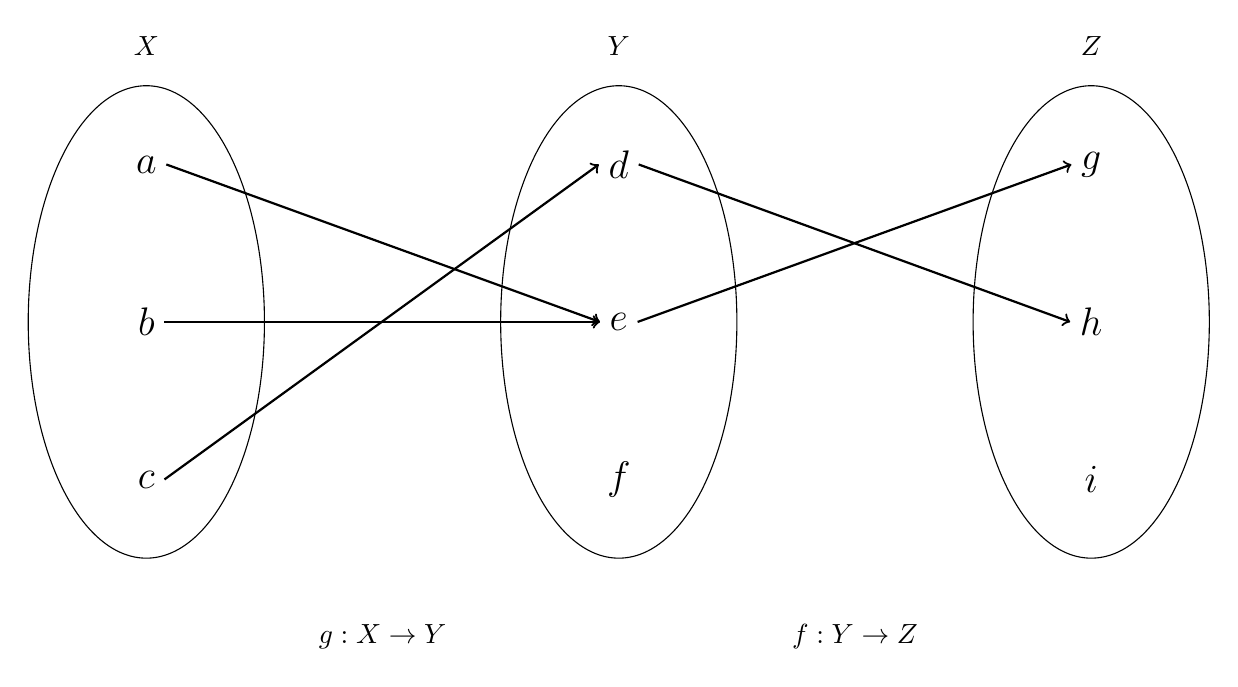
\begin{tikzpicture}
		\draw (-3,0) ellipse (1.5 and 3) node[yshift=3.5cm] {$X$};
		
		\draw (3,0) ellipse (1.5 and 3) node[yshift=3.5cm] {$Y$};
		
		\draw (9,0) ellipse (1.5 and 3) node[yshift=3.5cm] {$Z$};
				
		\node (a) at (-3,2) {\Large$a$};
		\node (b) at (-3,0) {\Large$b$};
		\node (c) at (-3,-2) {\Large$c$};
		
		\node (d) at (3,2) {\Large$d$};
		\node (e) at (3,0) {\Large$e$};
		\node (f) at (3,-2) {\Large$f$};
		
		\node (g) at (9,2) {\Large$g$};
		\node (h) at (9,0) {\Large$h$};
		\node (i) at (9,-2) {\Large$i$};
		
		\draw[thick,->] (a.east) -- (e.west);
		\draw[thick,->] (b.east) -- (e.west);
		\draw[thick,->] (c.east) -- (d.west);
		
		\draw[thick,->] (e.east) -- (g.west);
		\draw[thick,->] (d.east) -- (h.west);
		
		\draw (0,-4) node {$g:X\to Y$};
		\draw (6,-4) node {$f:Y\to Z$};
	\end{tikzpicture}}
	\caption{}
	\label{fig:comp}
\end{figure}

\begin{define}
	Define $f:Y\to Z$ and $g:X\to Y$. The composition of $f$ and $g$, notated as $f\circ g$ is a function $f\circ g:X\to Z$ such that $(f\circ g)(x)=f(g(x))$, or as seen in figure \eqref{fig:comp}.
\end{define}

An important property that's useful later is that functional composition is associative, or $f\circ (g\circ h)=(f\circ g) \circ h$. The proof is fairly trivial, so we ignore it here.

\begin{define}
\label{def:left}
	Define $f:X\to Y$. If there exists $g: Y\to X$ such that $g\circ f=I_X$, then $g$ is said to be the left inverse (retraction) of $f$.
\end{define}

$I_X$ in definition \eqref{def:left} is simpily the identity function on domain $X$, where $I_X(x)=x$. Like how the symbol 1 works with multiplication, any composition with the identity function results in the same function (e.g., $f\circ I=I\circ f=f$).
\begin{define}
	Define $f:X\to Y$. If there exists $g: Y\to X$ such that $f\circ g=I_Y$, then $g$ is said to be the right inverse (section) of $f$. 
\end{define}

The left inverse is illustrated by figure \eqref{fig:left}. As you can see, a left inverse, essentially \textit{retracts} the action of $f$ and sends everything back to where it came from.
\begin{figure}[h]
\centering
\resizebox{0.8\linewidth}{!}{
	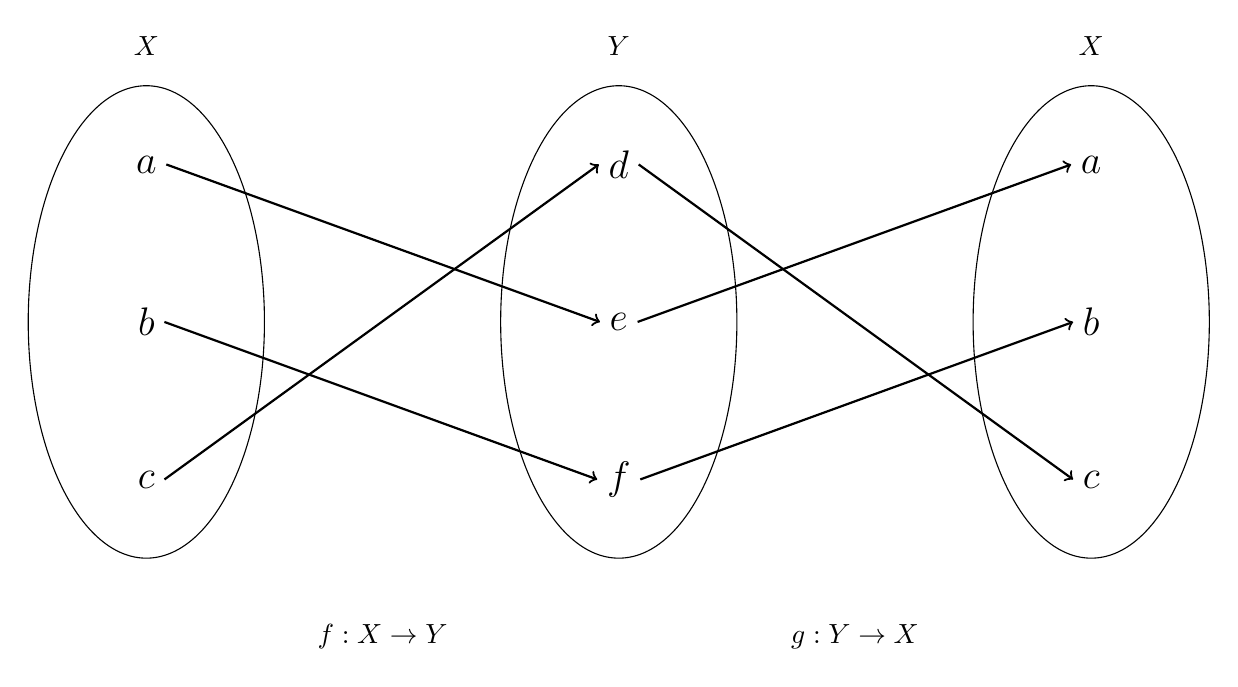
\begin{tikzpicture}
		\draw (-3,0) ellipse (1.5 and 3) node[yshift=3.5cm] {$X$};
		
		\draw (3,0) ellipse (1.5 and 3) node[yshift=3.5cm] {$Y$};
		
		\draw (9,0) ellipse (1.5 and 3) node[yshift=3.5cm] {$X$};
				
		\node (a) at (-3,2) {\Large$a$};
		\node (b) at (-3,0) {\Large$b$};
		\node (c) at (-3,-2) {\Large$c$};
		
		\node (d) at (3,2) {\Large$d$};
		\node (e) at (3,0) {\Large$e$};
		\node (f) at (3,-2) {\Large$f$};
		
		\node (g) at (9,2) {\Large$a$};
		\node (h) at (9,0) {\Large$b$};
		\node (i) at (9,-2) {\Large$c$};
		
		\draw[thick,->] (a.east) -- (e.west);
		\draw[thick,->] (b.east) -- (f.west);
		\draw[thick,->] (c.east) -- (d.west);
		
		\draw[thick,->] (e.east) -- (g.west);
		\draw[thick,->] (f.east) -- (h.west);
		\draw[thick,->] (d.east) -- (i.west);
		
		\draw (0,-4) node {$f:X\to Y$};
		\draw (6,-4) node {$g:Y\to X$};
	\end{tikzpicture}}
	\caption{}
	\label{fig:left}
\end{figure}

The right inverse, as seen in figure \eqref{fig:right}, can be thought of as a function that takes a \textit{section} of the domain of $f$ and reverses it.
\begin{figure}[h]
\centering
\resizebox{0.8\linewidth}{!}{
	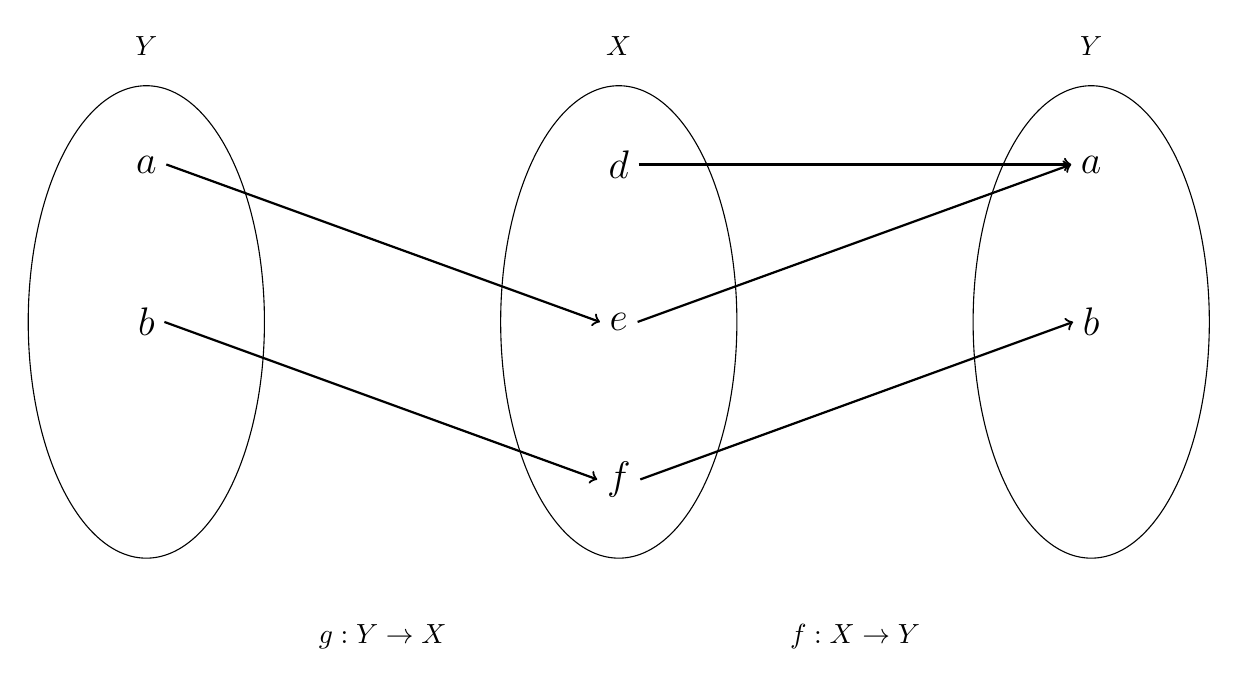
\begin{tikzpicture}
		\draw (-3,0) ellipse (1.5 and 3) node[yshift=3.5cm] {$Y$};
		
		\draw (3,0) ellipse (1.5 and 3) node[yshift=3.5cm] {$X$};
		
		\draw (9,0) ellipse (1.5 and 3) node[yshift=3.5cm] {$Y$};
				
		\node (a) at (-3,2) {\Large$a$};
		\node (b) at (-3,0) {\Large$b$};
		
		\node (d) at (3,2) {\Large$d$};
		\node (e) at (3,0) {\Large$e$};
		\node (f) at (3,-2) {\Large$f$};
		
		\node (g) at (9,2) {\Large$a$};
		\node (h) at (9,0) {\Large$b$};
		
		\draw[thick,->] (a.east) -- (e.west);
		\draw[thick,->] (b.east) -- (f.west);

		
		\draw[thick,->] (e.east) -- (g.west);
		\draw[thick,->] (f.east) -- (h.west);
		\draw[thick,->] (d.east) -- (g.west);
		
		\draw (0,-4) node {$g:Y\to X$};
		\draw (6,-4) node {$f:X\to Y$};
	\end{tikzpicture}}
	\caption{}
	\label{fig:right}
\end{figure}

Now that we've characterized these basic types of inverses let's start understanding these functions more with the following theorems.

\begin{theorem}
\label{thm:left}
Define $f:X\to Y$. If $f$ has a left inverse, then $f$ is one-to-one.	
\end{theorem}
\begin{proof}
	For any $x_1 x_2\in X$ such that $f(x_1)=f(x_2)$, let $g:Y\to X$ be the left inverse of $f$. Therefore, by the definition of the function, we have
	$$g(f(x_1))=g(f(x_2)).$$
	But since $g\circ f=I_x$, we deduce
	$$x_1=x_2$$
	hence $f$ is one-to-one.
\end{proof}

\begin{theorem}
\label{thm:right}
Define $f:X\to Y$. If $f$ has a right inverse, then $f$ is a surjection.\footnotemark
\end{theorem}
\footnotetext{The converse of theorems \eqref{thm:left} \eqref{thm:right} is also true, but proving them requires explicitly constructing a left or right inverse without making explicit assumptions about the underlying function, hence a bit tricky.}
\begin{proof}
Exercise.	
\end{proof}

\begin{define}
	Define $f:X\to Y$. If $f$ has left inverse $g: Y\to X$ and right inverse $h:y\to X$, then $f$ is said to have a two-sided inverse.
	$$f^{-1}=g=h$$
\end{define}
From here on out, I will use the term inverse for a two-sided inverse and specify when I only mean a left or right inverse.
\begin{theorem}
\label{thm:bi}
Suppose $f: X\to Y$ has an inverse, then $f$ is a bijection.\footnotemark
\end{theorem}
\footnotetext{Using the converse of theorem \eqref{thm:left} \eqref{thm:right}, we can also get the converse of this theorem.l}
\begin{proof}
	By theorems \eqref{thm:left} and \eqref{thm:right}, $f$ is both one-to-one and onto, concluding that $f$ is a bijection.
\end{proof}

Now, from theorem \eqref{thm:bi}, the function being a bijection is a necessary condition for the existence of an inverse. 
This means, that inverses only exist for functions if they are bijections, which might seem to contradict what you know about function inverses.\footnote{think of $\sin^{-1}(x)$ or $\cos^{-1}(x)$}
While this might be true by the strict definition of an inverse, there are ways to build meaningful inverses by changing the function definition just a bit. 
If this doesn't make sense to you, I will show in just a moment how this all makes sense.

\begin{define}
	Let $f:X\to Y$. Then we define $f| _A: A\to Y$, where
	$f|_A(a):=f(a)$, to be the \textbf{restriction of $f$ on $A$}
\end{define}
\begin{define}
	Let $f:X\to Y$. Then if $f|^B:X\to B$, where $f|^B(x):=f(x)$, is a well-defined function, then we call $f|^B$ the \textbf{corestriction of $f$ on $B$}.
\end{define}

We note that whilst the restriction of a function always exists, so long as $A$ is non-empty, the corestriction might not always be a well-defined function.
So, let's examine what guarantees the existence of $f|^B$.

\begin{lemma}
	Suppose $f:X\to Y$.
	$f|^B$ is well-defined if and only if $f(X)\subseteq B$.
	\label{lem:well-def-core}
\end{lemma}
\begin{proof}
	Suppose $f|^B$ is well-defined and let $y\in f(X)$.
	Then, by the definition of an image, there exists $x\in X$ such that $f(x)=y$. Then, by the definition of $f|^B$,
	$$f(x)=f|^B=y.$$
	Since $f|^B$ is well-defined, we have $y\in B$ implying $f(X)\subseteq B$.
	
	Then suppose $f(X)\subseteq B$. Then, we prove $f|^B$ is a well-defined function by checking with definition \eqref{def:function}.
	First, we check that $f|^B$ satisfies (1). This is done by noticing that for every $x\in X$, we have
	$$f|^B(x)=f(x)\in f(X)\subseteq B,$$
	hence $f|^B$ satisfies (1).
	
	To show $f|^B$ satisfies (2), we notice if $x_1,x_1\in X$$x_1=x_2$, we have
	$$f|^B(x_1):=f(x_1)=f|^B(x_2):=f(x_2).$$
	Since $f$ is a well-defined function, we have $x_1=x_2$.
\end{proof}


\begin{lemma}
For any $f:X\to Y$, there exists $f|^B$, $B\supseteq f(X)$, where $f|^B$ is a onto $B$.
\label{lem:co-onto}
\end{lemma}
\begin{proof}
	Let $B=f(X)$. By lemma \eqref{lem:well-def-core}, $f|^B$ is well-defined; hence it remains to show that $f|^B$ is onto $B$.
	By the definition of the image, for every $y\in B$, there exists $x\in X$ such that $f(x)=f|^B(x)=y$.
	Therefore, this suffices to prove $f|^B$ is onto $B$.
\end{proof}

\begin{lemma}
For any $f:X\to Y$, there exists $f|_A$, $A\subseteq X$	where $f|_A$ is one-to-one.
\label{lem:re-one}
\end{lemma}
\begin{proof}
	Define $C:P(X)\to X$, where $P(X)$ is the power set of $X$\footnote{or the set of all subsets of $X$} and for every $D\in P(X)$, $C(D)\in D.$
	We don't need to worry about the details of how $C$ is defined.
	We just care that such a function exists and is well-defined, which is guaranteed by the axiom of choice.\footnote{
	$C$ here is what we call a choice function. You can think of it as a map from a subset of $X$ to a corresponding element, or choice, within that subset.
	It's okay if you don't understand this and the axiom of choice. The only thing that's important here is that $C$ is a well-defined function, and it exists if we choose to believe in the axiom's validity}
	Let
	$$S:=\{f^{-1}(\{y\}):y\in Y\},$$
	where $S\subseteq P(X)$ since $f^{-1}(\{y\})\subseteq X$ for each $y\in Y$ by definition.
	Then let ${A:=C(S)}$.
	We wish to show this definition of $A$ makes $f|_A$ one-to-one.
	Suppose $x_1,x_1\in A$ such that
	$$f(x_1)=f(x_2).$$
	Since $x_1,x_2\in A$ hence $x_1,x_2\in C(S)$, there exists $y_1,y_2\in Y$ such that
	$$C(f^{-1}(\{y_1\})=x_1 \jand C(f^{-1}(\{y_2\})=x_2$$
	Then, by definition of $C$, we have
	$$x_1\in f^{-1}(\{y_1\}) \jand x_2\in f^{-1}(\{y_2\}).$$
	Therefore
	$$f(x_1)\in \{y_1\} \jand f(x_2)\in \{y_2\}$$
	hence
	$$f(x_1)=y_1 \jand f(x_2)=y_2.$$
	By assumption of $f(x_1)=f(x_2)$, we have $y_1=y_2$, hence
	$$f^{-1}(\{y_1\})=f^{-1}(\{y_2\}).$$
	Then, since $C$ is well-defined, we have 
	$$C(f^{-1}(\{y_1\})=C(f^{-1}(\{y_2\})$$
	hence $x_1=x_2$ therefore, $f|_A$ is one-to-one.
\end{proof}

\begin{theorem}
	Suppose $f:X\to Y$. Then there exists $A\subseteq X$ and $B\supseteq f(X)$ such that $f|^B_A$ is a bijection.
	\label{thm:to-bi}
\end{theorem}
\begin{proof}
	By lemmas \eqref{lem:co-onto} and \eqref{lem:re-one}, there exists $A$ and $B$ such that, $f|^B_A$ is one-to-one and onto $B$, hence $f|^B_A$ is a bijection.
\end{proof}

Now, with theorem \eqref{thm:to-bi}, we now know we can transform any function into a bijection, which has an inverse. With this, let's try this in an example.
\begin{ex}
	Let's try to construct a meaningful inverse for the function
	$$f(x)=\sqrt{x},$$
	where $f:[0,\infty)\to \real$.
	By imagining the function's plot in our heads, $f$ is one-to-one but isn't onto. Since we know $f$ doesn't output anything less than 0, we can construct a new function 
	$$g(x)=f(x)$$
	where $g:[0,\infty)\to [0,\infty)$. Now checking, $g$ is clearly onto since the range is exactly equal to the codomain, our new function $g$ is a bijection; therefore, there exists $g^{-1}$ such that
	$$g^{-1}\circ g=g\circ g^{-1}=I_{[0,\infty)}$$
	Doing some simple algebra, we get
	$$g^{-1}(x)=x^2.\footnotemark$$
	\footnotetext{Even though it's trivial, check this is indeed the case by computing $g^{-1}\circ g$ and $g\circ g^{-1}$.}
\end{ex}

\begin{ex}
	In this next example, let's try to determine the domain and codomain of $\sin^{-1}(x)$. By imagining the plot of $f(x)=\sin(x)$, we conclude that $f$ is not one-to-one nor onto. We first solve the "onto" problem by setting our new function's codomain to $f(X)$, which in this case is $[-1,1]$. 
	Like in the proof of theorem \eqref{lem:re-one}, there is a choice involved here, so unlike in the previous example, answers can vary depending on what we'd like to achieve.
	For our purposes, we will cut the number line, leaving the interval $(-\frac{\pi}{2},\frac{\pi}{2}]$.
	We can check this is the case by plotting $f$ on this domain, and $f$ clearly passes the horizontal line test. Hence we define $g: (-\frac{\pi}{2},\frac{\pi}{2}] \to [-1,1]$, where
	$$g(x)=\sin(x)$$
	and
	$$g^{-1}(x)=\sin^{-1}(x)$$
	where $g^{-1}: [-1,1] \to (-\frac{\pi}{2},\frac{\pi}{2}]$.
\end{ex}

\begin{ex}
	In this example, we'd like to find a meaningful inverse for
	$$f(x)=\frac{x}{1+x}$$
	on the largest possible domain $X$ such that $f$ is well-defined and a bijection. We conclude our largest possible domain for this function is $X=\{x\in\real: x\neq -1\}$.
	We do not yet have the tools to compute the image of $f$ under this domain directly so we will let $R$ represent this set hence
	$$f:\real \setminus \{-1\} \to R.$$
	Then, let us solve for the graph of $f^{-1}$ algebriclly. Let $y=f(x)$ for any $x$. Then
	$$y=\frac{x}{1+x}$$
	which by eliminating the dominator, we get
	$$y+xy=x$$
	hence
	$$y=x-xy$$
	$$y=x(1-y)$$
	$$x=\frac{y}{1-y}$$
	Then letting $f^{-1}(y)=x$, we conjecture the graph of $f^{-1}$ is
	$$f^{-1}(x)=\frac{x}{1-x}.\footnote{I just switch $x$ and $y$, for if anyone is confused. It just looks better this way. If you'd like, just substitute in $y$ to get $f^{-1}(y)$.}$$
	Being the inverse of $f$, we have $f^{-1}:R \to \real\setminus\{-1\}$.
	Since the maximum possible domain of $f^{-1}$ is $\real\setminus \{1\}$, we also conjecture
	$$R=\real\setminus \{1\}.$$
	First, we can check that $f$ is well defined with respect to our definition of $R$ by checking $f(x)\neq 1$ for any $x$ in our domain.
	To do this by way of contradiction. Thus if
	$$f(x)=\frac{x}{1+x}=1,$$
	then
	$$x=1+x$$
	implying $0=1$ which is a contradiction. Therefore, our definition of $f$ is well-defined.
	
	It remains to check that $f^{-1}$ is well-defined with respect to our codomain, that this is indeed the inverse of $f$, and that $f$ is a bijection.
	We check the first claim by checking that $f^{-1}$ doesn't output $-1$. Again, we proceed by contradiction hence, if there exists $x$ such that
	$$f^{-1}(x)=\frac{x}{1-x}=-1,$$
	then
	$$x=x-1$$
	implying $0=-1$ which is a contradiction.
	We check the remaining claims by computation.
	Since
	$$f(f^{-1}(x))=\frac{f^{-1}(x)}{1+f^{-1}(x)}=\frac{\frac{x}{1-x}}{1+\frac{x}{1-x}}$$
	$$=\frac{x}{(1-x)+x}=x=I$$
	and
	$$f^{-1}(f(x))=\frac{f(x)}{1-f(x)}=\frac{\frac{x}{1+x}}{1-\frac{x}{1+x}}$$
	$$=\frac{x}{(1+x)-x}=x=I$$
	we conclude that $f^{-1}$ indeed is an inverse, hence as a necessary condition, $f$ is a bijection.
	Therefore, the range of $f$ is exactly $R$ implying the range of $f$ is exactly $\real\setminus\{1\}$.
\end{ex}

\section{Exercies}
\noindent
1. Prove theorem \eqref{thm:oo}.

\noindent
2. Prove theorem \eqref{thm:right}.

\noindent
3. Determine, with proof whether the following functions are odd, even, or neither
\begin{enumerate}[label=\alph*)]
	\item $f(x)=\sqrt{x^4+x^2}+4$.
	\item $g(x)=x\sqrt{x^2+1}$.
\end{enumerate}

\noindent
4. Find two function $f, g$, even and odd respectively such that
$$f+g=x^2+2^x.$$

\noindent
5. For the following functions, determine the maximum possible domain without a calculator.
Then, when possible, construct an inverse without changing the domain of each function (you may need a graphing calculator for this second part).
\begin{enumerate}[label=\alph*)]
	\item $\frac{1}{\sqrt{1+x^2}}$.
	\item $\frac{x}{x^3+1}$.
	\item $\frac{2}{\sqrt{x-1}}$
\end{enumerate}









